%%%%%%%%%%%%%%%%%%%%%%%%%%%%%%%%%%%%%%%%%%%%%%%%%%%%%%%%%%%%%%%%%%%%%%%%%%%

\documentclass{standalone}

\usepackage{amsmath}
\usepackage{mathptmx}
\usepackage{pgfplots}
\usetikzlibrary{external}
\tikzexternalize{vapour-pressure-squared-errors}
\pgfplotsset{compat=1.15}

%% IEEE uses Times Roman font, so we'll default to Times.
%% These three commands make up the entire times.sty package.
\renewcommand{\rmdefault}{ptm}
\renewcommand{\ttdefault}{pcr}
\normalfont\selectfont

\begin{document}

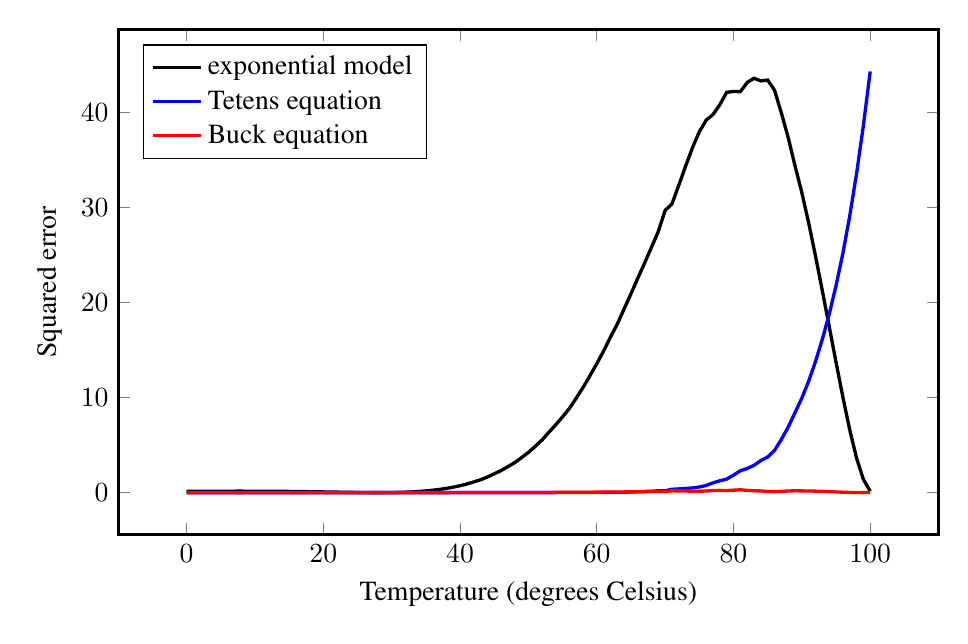
\begin{tikzpicture}
\tikzset{%%
  every mark/.append style={scale=1.0},%%
  scale=1.0%%
}
\pgfplotsset{%%
  every axis/.append style={font=\normalsize}%%
}
%%
\begin{axis}[%%
  axis line style=very thick,%%
  dotStyle/.style={very thick,mark=none},%%
  enlargelimits=true,%%
  height=8cm,%%
  legend cell align=left,%%
  legend pos=north west,%%
  width=12cm,%%
  %% x axis
  xlabel={\normalsize Temperature~(degrees~Celsius)},%%
  %% y axis
  ylabel={\normalsize Squared error},%%
  scaled y ticks=false,%%
  y tick label style=/pgf/number format/fixed%%
]
%%
%%
\addplot[dotStyle,black] coordinates {
  (0, 0.131834620866323)
  (1, 0.134439699701896)
  (2, 0.137845148740378)
  (3, 0.141477907866946)
  (4, 0.144777809769167)
  (5, 0.14797154716867)
  (6, 0.150565346462366)
  (7, 0.152098504905985)
  (8, 0.15215924306977)
  (9, 0.151959158210007)
  (10, 0.149655767878808)
  (11, 0.147358662908701)
  (12, 0.143371249082222)
  (13, 0.139133107331299)
  (14, 0.133132797216915)
  (15, 0.125487974977564)
  (16, 0.117778225067096)
  (17, 0.108154883580104)
  (18, 0.097675097679091)
  (19, 0.086733320352079)
  (20, 0.074103379224256)
  (21, 0.062096531016895)
  (22, 0.049746127742876)
  (23, 0.037820497079241)
  (24, 0.023201219436257)
  (25, 0.016255112784146)
  (26, 0.007927235684356)
  (27, 0.002216633699725)
  (28, 3.57776743951697E-06)
  (29, 0.002223951652992)
  (30, 0.009914980110289)
  (31, 0.02394277830453)
  (32, 0.046610137543362)
  (33, 0.07849793447354)
  (34, 0.121498913703669)
  (35, 0.178018551407446)
  (36, 0.248954250358515)
  (37, 0.336663290328387)
  (38, 0.44377471024737)
  (39, 0.571587826860293)
  (40, 0.725822188151092)
  (41, 0.904160977452151)
  (42, 1.1185055629026)
  (43, 1.35196926749242)
  (44, 1.64038937333086)
  (45, 1.9767924431746)
  (46, 2.31792714057662)
  (47, 2.73628930483096)
  (48, 3.15000478677741)
  (49, 3.67866244939463)
  (50, 4.23129149815705)
  (51, 4.86232669605269)
  (52, 5.54659534796302)
  (53, 6.35002719125014)
  (54, 7.13975231714954)
  (55, 7.97368927756436)
  (56, 8.8641063836989)
  (57, 9.95026782351692)
  (58, 11.0679932131495)
  (59, 12.2925069967878)
  (60, 13.5661874919183)
  (61, 14.8942951761966)
  (62, 16.3622930039245)
  (63, 17.7313641409256)
  (64, 19.3337810760261)
  (65, 20.9165812457444)
  (66, 22.5615295213435)
  (67, 24.1646101734374)
  (68, 25.8083001205217)
  (69, 27.4795247844578)
  (70, 29.7032787394522)
  (71, 30.3870830709397)
  (72, 32.3448528096479)
  (73, 34.3656954987244)
  (74, 36.2982781658824)
  (75, 37.9718055803913)
  (76, 39.2003503274549)
  (77, 39.7907995887876)
  (78, 40.8225620961427)
  (79, 42.1287884595735)
  (80, 42.2212695934644)
  (81, 42.195808181838)
  (82, 43.1605594487266)
  (83, 43.6107790590798)
  (84, 43.3299575113624)
  (85, 43.4231003579192)
  (86, 42.3611359801396)
  (87, 39.9732557483883)
  (88, 37.3818559314281)
  (89, 34.4078395598176)
  (90, 31.5810340705433)
  (91, 28.3806066126438)
  (92, 24.9001075062269)
  (93, 21.2385013716818)
  (94, 17.5006737136832)
  (95, 13.724298830696)
  (96, 10.0611972585274)
  (97, 6.62832135210835)
  (98, 3.65310767618065)
  (99, 1.39389115452642)
  (100, 0.144789704638064)
};
\addlegendentry{exponential model}
%%
%%
%% The Tetens equation.
\addplot[dotStyle,blue] coordinates {
  (0, 5.01615593112191E-06)
  (1, 1.79418073858415E-07)
  (2, 1.99473406056781E-06)
  (3, 2.11754041057895E-06)
  (4, 1.49489263854119E-06)
  (5, 1.05952174492292E-07)
  (6, 4.72603938513236E-07)
  (7, 1.7724225498269E-06)
  (8, 1.40932062071692E-06)
  (9, 3.62553298906801E-06)
  (10, 1.44359507525643E-06)
  (11, 3.50120875973621E-06)
  (12, 3.16631159613101E-06)
  (13, 8.23400323632463E-06)
  (14, 1.00092349923384E-05)
  (15, 7.65030209517887E-06)
  (16, 1.49273933809842E-05)
  (17, 1.39166536606112E-05)
  (18, 1.39049067930831E-05)
  (19, 1.85949418409123E-05)
  (20, 9.16316764574214E-06)
  (21, 1.23649235101848E-05)
  (22, 1.24003915420284E-05)
  (23, 1.50900395703519E-05)
  (24, 4.15771348324099E-05)
  (25, 1.27871739914201E-05)
  (26, 9.72031497305532E-06)
  (27, 6.00424664349545E-06)
  (28, 3.84541474014807E-06)
  (29, 1.33131604999579E-06)
  (30, 4.26301231222037E-07)
  (31, 1.45148166632755E-06)
  (32, 1.01605611021764E-07)
  (33, 8.42182943333466E-07)
  (34, 2.13496161064405E-06)
  (35, 7.20586236854005E-06)
  (36, 1.01505515246928E-05)
  (37, 1.17312039148965E-05)
  (38, 1.38256363296585E-05)
  (39, 1.04773628436713E-05)
  (40, 1.60309320698769E-05)
  (41, 8.35811599249386E-06)
  (42, 2.13076871453799E-05)
  (43, 6.79591296955978E-08)
  (44, 7.08245555914914E-06)
  (45, 5.80532829446078E-05)
  (46, 1.73054110086667E-06)
  (47, 5.80058972577581E-08)
  (48, 0.000237981337655)
  (49, 0.000177365108981)
  (50, 0.0004217883205)
  (51, 0.0005707160158)
  (52, 0.000921886789979)
  (53, 0.000736122405319)
  (54, 0.001727404582207)
  (55, 0.003746981266293)
  (56, 0.007028787920247)
  (57, 0.007637310502149)
  (58, 0.010006013201324)
  (59, 0.012125091990878)
  (60, 0.015929638822311)
  (61, 0.021640271936152)
  (62, 0.026175755201944)
  (63, 0.039789331600962)
  (64, 0.048218766037002)
  (65, 0.063397458607332)
  (66, 0.081770170691052)
  (67, 0.110353617319846)
  (68, 0.145046315043813)
  (69, 0.187049520041104)
  (70, 0.191787158431007)
  (71, 0.346014431244839)
  (72, 0.390214259410229)
  (73, 0.434017043828559)
  (74, 0.493371194538504)
  (75, 0.58909284849262)
  (76, 0.750741746745747)
  (77, 1.02362492689629)
  (78, 1.24591032714508)
  (79, 1.42302313791718)
  (80, 1.83652680652509)
  (81, 2.3002161475741)
  (82, 2.5317962984956)
  (83, 2.86583294497433)
  (84, 3.37167379776548)
  (85, 3.74756569151456)
  (86, 4.43863754198021)
  (87, 5.58993142488436)
  (88, 6.88482194148604)
  (89, 8.41817734297706)
  (90, 9.94120399273977)
  (91, 11.730474380422)
  (92, 13.7948677750482)
  (93, 16.1400257725513)
  (94, 18.7682770733164)
  (95, 21.7720810147472)
  (96, 25.1684957097309)
  (97, 29.0815823946385)
  (98, 33.5507766734836)
  (99, 38.618074663661)
  (100, 44.3287385226981)
};
\addlegendentry{Tetens equation}
%%
%%
%% The Buck equation.
\addplot[dotStyle,red] coordinates {
  (0, 2.98657001437116E-05)
  (1, 5.72640919359421E-06)
  (2, 9.82498518568842E-07)
  (3, 2.86466525151749E-07)
  (4, 1.28890083820244E-07)
  (5, 7.34224519401817E-07)
  (6, 2.20644672935504E-06)
  (7, 3.11736704951777E-06)
  (8, 1.65080994650196E-06)
  (9, 2.88661542751973E-06)
  (10, 5.39705659565686E-07)
  (11, 1.41875646186732E-06)
  (12, 8.88799965692353E-07)
  (13, 3.76810135034116E-06)
  (14, 4.9166861648855E-06)
  (15, 3.55010057765314E-06)
  (16, 9.8499686121909E-06)
  (17, 1.06505541922676E-05)
  (18, 1.31868004843302E-05)
  (19, 2.21387146066411E-05)
  (20, 1.63353330811963E-05)
  (21, 2.80226039340846E-05)
  (22, 3.85907535684735E-05)
  (23, 5.85114414540905E-05)
  (24, 2.07220951982409E-06)
  (25, 0.000100142352761)
  (26, 0.000124522198038)
  (27, 0.000151209637497)
  (28, 0.000190846332548)
  (29, 0.000231746707072)
  (30, 0.000294165791593)
  (31, 0.000414083128765)
  (32, 0.000470481516758)
  (33, 0.000584497815488)
  (34, 0.000725544635598)
  (35, 0.000854413091661)
  (36, 0.001053325412904)
  (37, 0.001306245886893)
  (38, 0.001597052333812)
  (39, 0.002000952702791)
  (40, 0.002343235922565)
  (41, 0.002926120919771)
  (42, 0.003254400392951)
  (43, 0.004445680050566)
  (44, 0.004698021418158)
  (45, 0.004673928762318)
  (46, 0.006728638733824)
  (47, 0.007322459528107)
  (48, 0.01106773232965)
  (49, 0.011513171841949)
  (50, 0.01401980241381)
  (51, 0.015684682759393)
  (52, 0.018141900940255)
  (53, 0.017911868132526)
  (54, 0.022475407779252)
  (55, 0.029026460567638)
  (56, 0.037176217104987)
  (57, 0.038040374829591)
  (58, 0.042044020517583)
  (59, 0.044526808463899)
  (60, 0.048980804887749)
  (61, 0.055001022412091)
  (62, 0.057312976036234)
  (63, 0.070181068011319)
  (64, 0.073028396717249)
  (65, 0.081073114373027)
  (66, 0.088791939988982)
  (67, 0.102245846544708)
  (68, 0.115642315304107)
  (69, 0.128946110159967)
  (70, 0.107097698221219)
  (71, 0.189391137348464)
  (72, 0.179549107701742)
  (73, 0.163168666292669)
  (74, 0.149843031396315)
  (75, 0.147988101841811)
  (76, 0.166830878858481)
  (77, 0.221189184063579)
  (78, 0.23273941634193)
  (79, 0.209038748702295)
  (80, 0.257304924056979)
  (81, 0.297467839267763)
  (82, 0.234970633165398)
  (83, 0.192321156824326)
  (84, 0.176696487100934)
  (85, 0.118280865314747)
  (86, 0.104479615199873)
  (87, 0.138764752047445)
  (88, 0.16500310865837)
  (89, 0.192720362061736)
  (90, 0.181312380176567)
  (91, 0.169563271770464)
  (92, 0.153898932904997)
  (93, 0.131754686950266)
  (94, 0.102190095115019)
  (95, 0.072069016172247)
  (96, 0.042292228785025)
  (97, 0.018989647255369)
  (98, 0.003806306079858)
  (99, 0.000658313699937)
  (100, 0.016131262356405)
};
\addlegendentry{Buck equation}
\end{axis}
\end{tikzpicture}

\end{document}
